\clearpage
\chapter{MATLAB Problem 2.3}

\paragraph{a)}

In den Plots ist deutlich ersichtlich, dass $\mu$ direkt in die Zeitkonstanten, also in die
Konvergenzgeschwindigkeit einflie�t. Im Falle von zero-mean White-Noise sind alle Eigenwerte der
Autokorrelationsmatrix 1. Somit ergeben sich die Zeitkonstanten theoretisch: $\approx \frac{1}{\mu \lambda_k} = \frac{1}{\mu}$.
Diese Formel stimmte auch sehr gut mit den aus den Plots ermittelten Werten f�r $\tau_k$ �berein.
Wie in der Abbildung \ref{fig:2_3_a_1} zu sehen, ist der Algorithmus bei $\mu=1$ im Falle des LMS instabil.
Der Misalignmentvector divergiert und der MSE wird immer gr��er.
Beim NLMS und $\mu=1$ ist keine deutliche Konvergenz des Misalignmentvectors ersichtlich. Der Misalignmentvector
divergiert allerdings auch nicht so wie beim LMS(ohne Normalisierung). Der Grund hierf�r ist, dass $\mu$ durch
$\vm{x}[n]$ dividiert wird und somit etwas kleiner ist. $\mu$ ist aber dennoch zu gro� um die Koeffizienten vern�nftig
anzun�hern.


F�r ein gr��eres $\mu$ konvergiert der MSE wesentlich schneller gegen sein Minimum, allerdings ist auch
der Excess-Error etwas gr��er.

Beim NLMS wird $\mu$ durch $|\vm{x}[n]|^2$ dividiert. Bei einer Varianz von 1 und einer Filterordnung $N=3$ ist
der tapped input Vektor $\vm{x}[n]$ 3 Elemente gro�. Somit ergibt sich ein Erwartungswert f�r $\vm{x}[n]$ von 3.
Aus diesem Grund sind die Zeitkonstanten f�r diese Eingangsvarianz um den Faktor 3 gr��er. Der entscheidende Vorteil
beim LMS ist jetzt, dass die Konvergenzgeschwindigkeit nicht mehr von der Eingangsvarianz abh�ngt. Diese
ist im n�chsten Abschnitt zu sehen.

\begin{figure}[ht!]
 \centering
 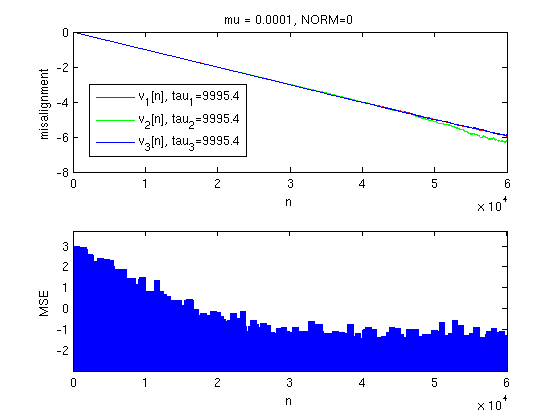
\includegraphics[width=12cm]{./plots/2_3_a_0_0001.png}
 % 2_3_a_0_0001.png: 560x420 pixel, 90dpi, 15.81x11.85 cm, bb=
 \caption{LMS, $\mu=0.0001$, zero-mean unit variance white noise input}
 \label{fig:2_3_a_0_0001}
\end{figure}

\begin{figure}[ht!]
 \centering
 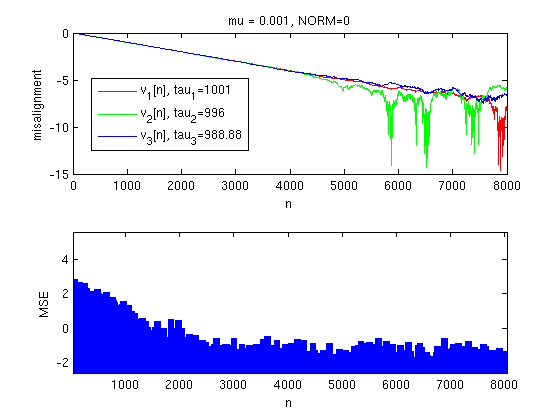
\includegraphics[width=12cm]{./plots/2_3_a_0_001.png}
 % 2_3_a_0_0001.png: 560x420 pixel, 90dpi, 15.81x11.85 cm, bb=
 \caption{LMS, $\mu=0.001$, zero-mean unit variance white noise input}
 \label{fig:2_3_a_0_001}
\end{figure}

\begin{figure}[ht!]
 \centering
 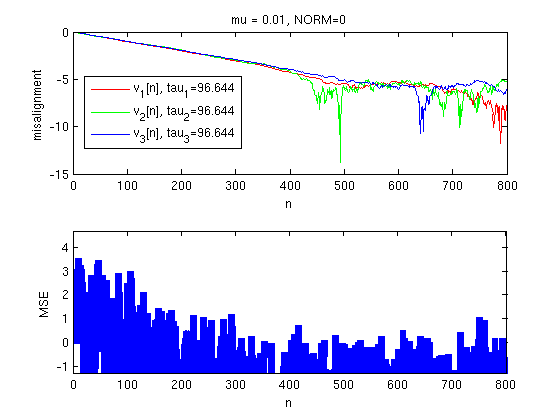
\includegraphics[width=12cm]{./plots/2_3_a_0_01.png}
 % 2_3_a_0_0001.png: 560x420 pixel, 90dpi, 15.81x11.85 cm, bb=
 \caption{LMS, $\mu=0.01$, zero-mean unit variance white noise input}
 \label{fig:2_3_a_0_01}
\end{figure}

\begin{figure}[ht!]
 \centering
 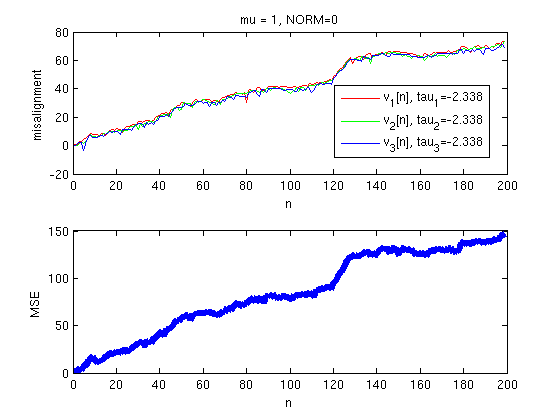
\includegraphics[width=12cm]{./plots/2_3_a_1.png}
 % 2_3_a_0_0001.png: 560x420 pixel, 90dpi, 15.81x11.85 cm, bb=
 \caption{LMS, $\mu=1$, zero-mean unit variance white noise input}
 \label{fig:2_3_a_1}
\end{figure}

%NLMS:
\begin{figure}[ht!]
 \centering
 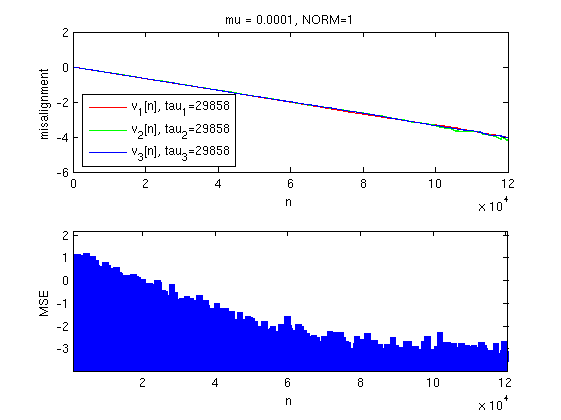
\includegraphics[width=12cm]{./plots/2_3_a_0_0001_norm.png}
 % 2_3_a_0_0001.png: 560x420 pixel, 90dpi, 15.81x11.85 cm, bb=
 \caption{NLMS, $\mu=0.0001$, zero-mean unit variance white noise input}
 \label{fig:2_3_a_0_0001_norm}
\end{figure}

\begin{figure}[ht!]
 \centering
 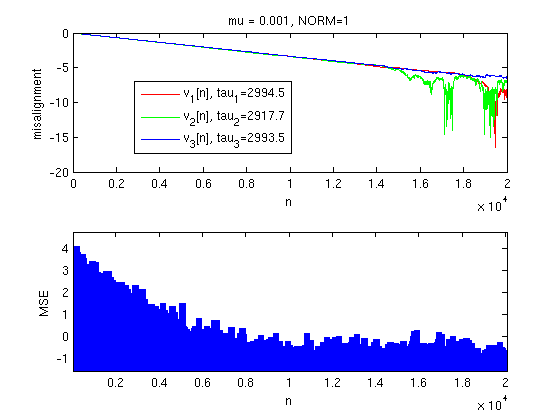
\includegraphics[width=12cm]{./plots/2_3_a_0_001_norm.png}
 % 2_3_a_0_0001.png: 560x420 pixel, 90dpi, 15.81x11.85 cm, bb=
 \caption{NLMS, $\mu=0.001$, zero-mean unit variance white noise input}
 \label{fig:2_3_a_0_001_norm}
\end{figure}

\begin{figure}[ht!]
 \centering
 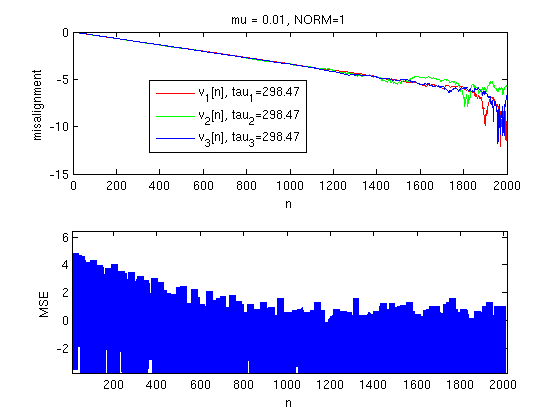
\includegraphics[width=12cm]{./plots/2_3_a_0_01_norm.png}
 % 2_3_a_0_0001.png: 560x420 pixel, 90dpi, 15.81x11.85 cm, bb=
 \caption{NLMS, $\mu=0.01$, zero-mean unit variance white noise input}
 \label{fig:2_3_a_0_01_norm}
\end{figure}

\begin{figure}[ht!]
 \centering
 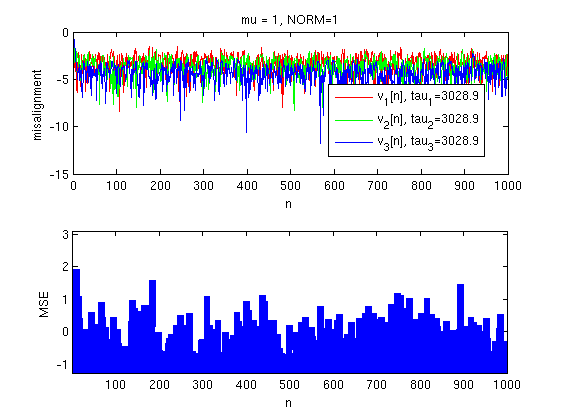
\includegraphics[width=12cm]{./plots/2_3_a_1_norm.png}
 % 2_3_a_0_0001.png: 560x420 pixel, 90dpi, 15.81x11.85 cm, bb=
 \caption{NLMS, $\mu=1$, zero-mean unit variance white noise input}
 \label{fig:2_3_a_1_norm}
\end{figure}

\clearpage

\paragraph{b)}

In den Plots wird ersichtlich, dass die Konvergenzgeschwindigkeit des LMS von der Varianz des Eingangssingals
abh�ngt. Somit Konvergiert dieser Algorithmus bei einer gr��eren Varianz von $\vm{x}[n]$ schneller, bzw. bei einer
sehr geringen Eingangsvarianz nur sehr gering. Um das ganze noch mit zahlen zu belegen, betrachten wir zun�chst
wieder die Formel f�r die Zeitkonstanten: $\tau_k \approx \frac{1}{\mu \lambda_k}$. Da es sich wieder um
wei�es Rauschen handelt, sind alle Eigenwerte $\lambda_k$ gleich und entsprechen der Varianz.
Somit ergibt sich bei einer Eingangsvarianz von $1.5$ theoretisch eine Zeitkonstante von $1/(1.5\mu) \approx 0.666/\mu$.
Diese Werte k�nnen sehr gut anhand der Plots abgelesen werden.

Beim NLMS hat die Eingangsvarianz keinen Einfluss da $\mu$ entsprechend der Eingangsvarianz angepasst wird.
Dies ist sehr gut anhand der berechneten Zeitkonstanten in den Abbildungen \ref{fig:2_3_b_xvar_0_2_norm} und \ref{fig:2_3_b_xvar_1_5_norm}
zu sehen.

\begin{figure}[ht!]
 \centering
 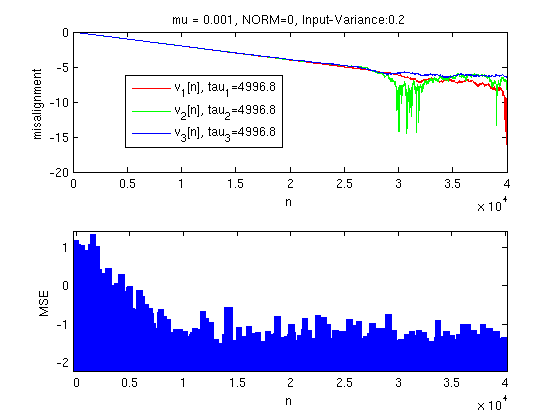
\includegraphics[width=12cm]{./plots/2_3_b_xvar_0_2.png}
 % 2_3_a_0_0001.png: 560x420 pixel, 90dpi, 15.81x11.85 cm, bb=
 \caption{LMS, $\mu=0.001$, zero-mean white noise input with variance=$0.2$}
 \label{fig:2_3_b_xvar_0_2}
\end{figure}

\begin{figure}[ht!]
 \centering
 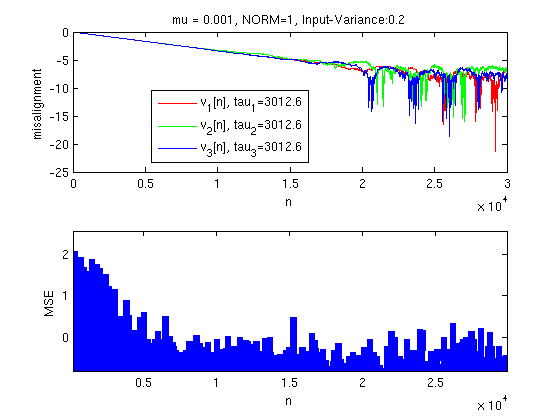
\includegraphics[width=12cm]{./plots/2_3_b_xvar_0_2_norm.png}
 % 2_3_a_0_0001.png: 560x420 pixel, 90dpi, 15.81x11.85 cm, bb=
 \caption{NLMS, $\mu=0.001$, zero-mean white noise input with variance=$0.2$}
 \label{fig:2_3_b_xvar_0_2_norm}
\end{figure}

\begin{figure}[ht!]
 \centering
 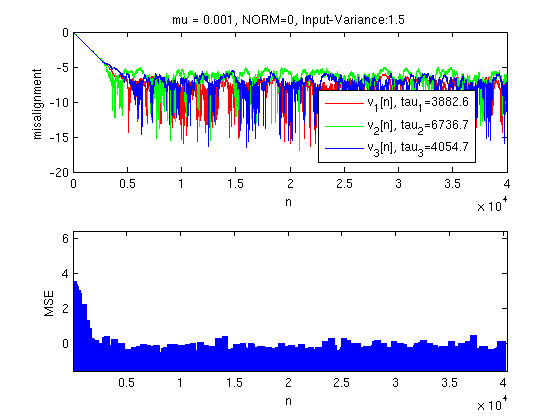
\includegraphics[width=12cm]{./plots/2_3_b_xvar_1_5.png}
 % 2_3_a_0_0001.png: 560x420 pixel, 90dpi, 15.81x11.85 cm, bb=
 \caption{LMS, $\mu=0.001$, zero-mean white noise input with variance=$1.5$}
 \label{fig:2_3_b_xvar_1_5}
\end{figure}

\begin{figure}[ht!]
 \centering
 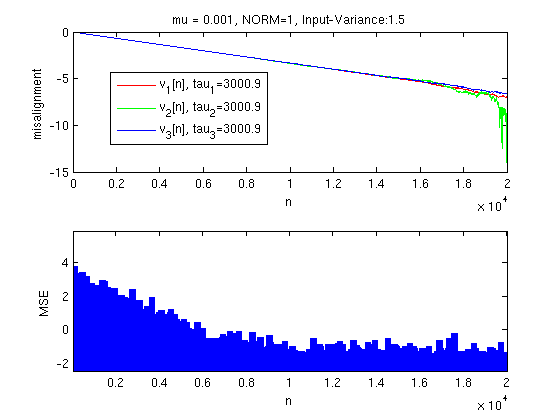
\includegraphics[width=12cm]{./plots/2_3_b_xvar_1_5_norm.png}
 % 2_3_a_0_0001.png: 560x420 pixel, 90dpi, 15.81x11.85 cm, bb=
 \caption{NLMS, $\mu=0.001$, zero-mean white noise input with variance=$1.5$}
 \label{fig:2_3_b_xvar_1_5_norm}
\end{figure}


\paragraph{c)}

Da das Eingangssignal jetzt kein Wei�es Rauschen mehr ist, sind die Eigenwerte von $\vm{R}_{xx}$ nicht mehr gleich.
Dadurch konvergieren die Komponenten von $v$ unterschiedlich schnell.

Der MSE nimmt kontinuierlich ab, bis er den noise-floor erreicht (MMSE + excess-error).

\begin{figure}[ht!]
 \centering
 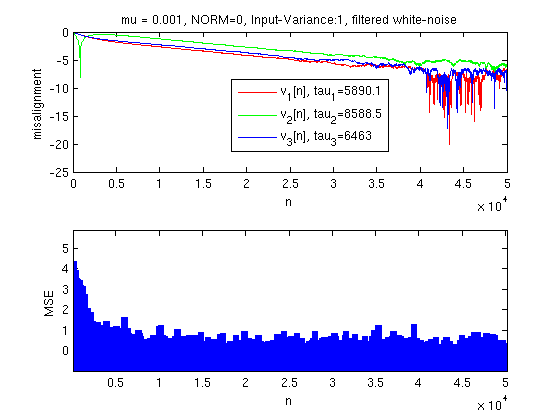
\includegraphics[width=12cm]{./plots/2_3_c.png}
 % 2_3_a_0_0001.png: 560x420 pixel, 90dpi, 15.81x11.85 cm, bb=
 \caption{LMS, $\mu=0.001$, zero-mean white noise input with variance=$1$, filtered}
 \label{fig:2_3_c}
\end{figure}

\begin{figure}[ht!]
 \centering
 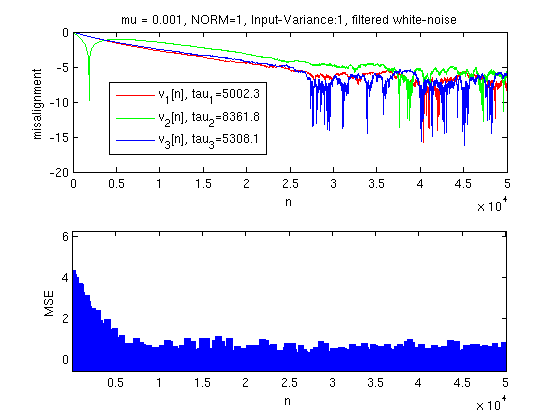
\includegraphics[width=12cm]{./plots/2_3_c_norm.png}
 % 2_3_a_0_0001.png: 560x420 pixel, 90dpi, 15.81x11.85 cm, bb=
 \caption{NLMS, $\mu=0.001$, zero-mean white noise input with variance=$1$, filtered}
 \label{fig:2_3_c}
\end{figure}


\paragraph{d)}
Der MSE nimmt kontinuierlich ab, bis er den noise-floor erreicht (MMSE + excess-error).

\paragraph{e)}

Berechnung des Excess Errors:
Wie in der Vorlesung vom 18.11.2011 hergeleitet ergibt sich der Excess Error wie folgt:

\begin{equation}
 M \cdot MMSE
\end{equation}

Wobei $M$ als Misadjustment bezeichnet wird

\begin{equation}
 M = \frac{\mu ||\vm{x[n]}||^2}{2-\mu ||\vm{x[n]}||^2}
\end{equation}
Wobei $\vm{x[n]}||^2$ Der Varianz des Eingangssingals entspricht.

Das Minimum der Kostenfunktion(=MMSE) (siehe Gleichung \ref{eq:cost3} wurde wie folgt ermittelt:

\begin{equation}
MMSE = \sigma_v^2 - \vm{p}^T\vm{R}_{xx}^{-1}\vm{p}
\label{eq:bla}
\end{equation}

Formt man nun die Wiener Hopf Solution auf $\vm{p}$ um so erh�lt man:
$\vm{p} = \vm{R}_{xx}\vm{h}$. In die Gleichung \ref{eq:bla} eingesetzt ergibt das (f"ur white noise!!!):

\begin{equation}
MMSE = \sigma_v^2 - \vm{h}^T\vm{R}_{xx}^T \vm{R}_{xx}^{-1} \vm{R}_{xx}\vm{h} = \sigma_v^2 -\vm{h}^T\vm{R}_{xx}^T\vm{h}
= \sigma_v^2 - ||h||\sigma_x^2
\label{eq:bla1}
\end{equation}

\begin{equation}
 excess error = MMSE \cdot M
\end{equation}


Nun ergeben sich folgende Werte f�r den Excesserror in dB:\\


\begin{table}[!htp]
\begin{center}
\begin{tabular}
{| c || c | c | c | c | c |}   %  || zur Unterteilung eingestellte/gemnessene/berechnete Werte
\hline
Eingangs-Varianz $\sigma_x^2$ & $\mu = 0.0001$ & $\mu = 0.001$ & $\mu = 0.01$ & $\mu = 1$ \\ \hline \hline
1 & -44.31 & -34.31 & -24.31 & -4.31 \\ \hline
1.5 &  -40.7786 & -30.7786 & -20.7786 &  -0.7786 \\ \hline
0.2 & -58.4873 & -48.4873 & -38.4873 & -18.4873 \\ \hline
\end{tabular}
\caption{Ermittelten Werte f�r den Excess-Error in dB beim LMS}
\end{center}
\end{table}

\begin{table}[!htp]
\begin{center}
\begin{tabular}
{| c || c | c | c | c | c |}   %  || zur Unterteilung eingestellte/gemnessene/berechnete Werte
\hline
Eingangs-Varianz $\sigma_x^2$ & $\mu = 0.0001$ & $\mu = 0.001$ & $\mu = 0.01$ & $\mu = 1$ \\ \hline \hline
1 & -49.0873 & -39.0873 & -29.0873  & -9.0873 \\ \hline
1.5 &  -45.5498 & -35.5498 & -25.5498 &  -5.5498 \\ \hline
0.2 & -63.2585 & -53.2585 & -43.2585 & -23.2585 \\ \hline
\end{tabular}
\caption{Ermittelten Werte f�r den Excess-Error in dB beim NLMS}
\end{center}
\end{table}

Wie bereits erkl"art nimmt der Excesserror bei einem kleinerem $\mu$ ab. Bei einer kleineren Eingangsvarianz
ist der Excesserror auch kleiner. Da beim NLMS das effektive $\mu$ verkleinert wird, ist bei dieser Variante des
LMS der Excesserror etwas geringer.
